\documentclass{article}
\usepackage{hyperref}
\usepackage{amsmath}
\usepackage{graphicx} % Required for inserting images
\usepackage{subcaption} %  for subfigures environments
\usepackage{float}

\title{Path tracer}
\author{Javier Sancho Olano \\ \href{mailto:815520@unizar.es}{815520@unizar.es}}
\date{Enero 2024}

\begin{document}

\maketitle

\tableofcontents
\newpage

\section{Introducción}
La ecuación de render es una ecuación integral que describe la cantidad de
radiancia emitida de un punto \(\mathbf{x}\) de una superficie hacia una
dirección \(\mathbf{\omega_{o}}\)

\begin{equation}
  L_o(\mathbf{x}, \mathbf{\omega_{o}}) = L_e(\mathbf{x}, \mathbf{\omega_{o}}) + \int_{\Omega} L_i(\mathbf{x}, \mathbf{\omega_{i}}) \cdot f_r(\mathbf{x}, \mathbf{\omega_{i}}, \mathbf{\omega_{o}}) \cdot  |\mathbf{n} \cdot \mathbf{\omega_{i}}| \, d\omega_{i}
\end{equation}

\begin{figure}[h]
  \centering 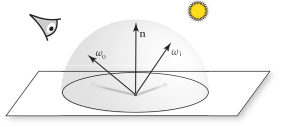
\includegraphics[width=0.6\textwidth]{imgs/rendereq.png}
  \caption{Ilustración del problema de la ecuación de render}
\end{figure}

donde:
\begin{itemize}
  \item \(\mathbf{x}\) es un punto en el espacio
  \item \(\mathbf{\omega_{o}}\) es la direccion de salida
  \item \(\mathbf{n}\) es la normal de la superficie
  \item \(\mathbf{\omega_{i}}\) es la dirección de la radiancia incidente
  \item \(L_o(\mathbf{x}, \mathbf{\omega_{o}})\) es la cantidad de radiancia
        emitida de un punto \(\mathbf{x}\) de una superficie hacia una dirección
        \(\mathbf{\omega_{o}}\)
  \item \(L_e(\mathbf{x}, \mathbf{\omega_{o}})\) es la radiancia que la
        superficie emite en el punto \(\mathbf{x}\), hacia
        \(\mathbf{\omega_{o}}\)
  \item \(\int_{\Omega} ... \, d\omega_{i}\) es una integral sobre la hemiesfera
        \(\Omega\)
  \item \(L_i(\mathbf{x}, \mathbf{\omega_{i}}) \) es la radiancia incidente en
        \(\mathbf{x}\) desde la dirección \(\mathbf{\omega_{i}}\)
  \item \(f_r(\mathbf{x}, \mathbf{\omega_{i}}, \mathbf{\omega_{o}}) \) es la
        BTDF, la proporción de radiancia reflejada hacia \(\mathbf{\omega_{o}}\)
        desde \(\mathbf{\omega_{i}}\) en el punto \(\mathbf{x}\)
  \item \(|\mathbf{n} \cdot \mathbf{\omega_{i}}|\) a.k.a \(\cos\theta_{i}\) es
        el factor que ajusta la contribución de la radiancia incidente respecto
        a \(\mathbf{\omega_{i}}\)
\end{itemize}

Entonces \textit{path tracer} hace referencia a la técnica que se usará para
resolver esta ecuación. El algoritmo \textit{path tracer} usará el estimador de
Monte Carlo para aproximar la integral de render.

Si quisiéramos evaluar una integral como esta \(\int^{b}_{a} f(x) \; dx\), y
dado una variable aleatoria uniforme \(X_{i} \in [a, b]\), el estimador de Monte
Carlo dice que la esperanza del siguiente estimador, \(E[F_{N}]\) es igual a la
integral.
\[F_{N}=\frac{b-a}{N} \sum_{i=1}^{N} f(X_{i}) \]
\[E[F_{N}]= \int^{b}_{a} f(x) \; dx\]

Si la variable aleatoria \(X_{i}\) se extrae de una PDF arbitraria entonces, la
esperanza del siguiente estimador sigue siendo la integral.
\begin{equation}
  F_{N}=\frac{1}{N} \sum_{i=1}^{N} \frac{f(X_{i})}{p(X_{i})}
\end{equation}
\begin{equation}
  E[F_{N}]= \int^{b}_{a} f(x) dx
\end{equation}

Aplicandolo la ecuacion 2 a nuestra ecuación de render (Eq. 1):

\begin{equation}
  L_o(\mathbf{x}, \mathbf{\omega_{o}}) \approx L_e(\mathbf{x}, \mathbf{\omega_{o}}) + \frac{1}{N} \sum_{i=1}^{N} \frac{L_i(\mathbf{x}, \mathbf{\omega_{i}}) \cdot f_r(\mathbf{x}, \mathbf{\omega_{i}}, \mathbf{\omega_{o}}) \cdot  |\mathbf{n} \cdot \mathbf{\omega_{i}}|}{p(\omega_{i})}
\end{equation}

Para un camino (\(N=1\))
\(\{\mathbf{x_{1}}, \mathbf{x_{2}}, ..., \mathbf{x_{k}}\}\),
\(L_{i}(\mathbf{x_{j}}, \mathbf{\omega_{o}})=L_{o}(\mathbf{x_{j+1}}, \mathbf{\omega_{o}})\)
y cuando la superficie emita, simplificaremos:
\(L_{o}(\mathbf{x}, \mathbf{\omega_{o}})=L_{e}(\mathbf{x}, \mathbf{\omega_{o}})\)

Podemos descomponer la radiancia incidente en dos componentes:
\[L_i(\mathbf{x}, \mathbf{\omega_{i}}) = L_{i,d}(\mathbf{x}, \mathbf{\omega_{i}}) + L_{i,i}(\mathbf{x}, \mathbf{\omega_{i}}),\]

\begin{itemize}
  \item \(L_{i,d}(\mathbf{x}, \mathbf{\omega_{i}})\) es la radiancia directa que
        llega a \(\mathbf{x}\) desde una fuente de luz
  \item \(L_{i,i}(\mathbf{x}, \mathbf{\omega_{i}})\) es la radiancia indirecta
        que llega a \(\mathbf{x}\) tras haber sido reflejada o refractada.
\end{itemize}

Por lo que la ecuacion de render se puede reescribir como:

\begin{equation}
  \begin{split}
    L_o(\mathbf{x}, \mathbf{\omega_{o}}) & = L_e(\mathbf{x}, \mathbf{\omega_{o}}) + \int_{\Omega} (L_{i,d}(\mathbf{x}, \mathbf{\omega_{i}}) + L_{i,i}(\mathbf{x}, \mathbf{\omega_{i}})) \cdot f_r(\mathbf{x}, \mathbf{\omega_{i}}, \mathbf{\omega_{o}}) \cdot  |\mathbf{n} \cdot \mathbf{\omega_{i}}| \, d\omega_{i} \\
                                         & = L_e(\mathbf{x}, \mathbf{\omega_{o}})
                                           + \int_{\Omega} L_{i,d}(\mathbf{x}, \mathbf{\omega_{i}}) \cdot f_r(\mathbf{x}, \mathbf{\omega_{i}}, \mathbf{\omega_{o}}) \cdot  |\mathbf{n} \cdot \mathbf{\omega_{i}}| \, d\omega_{i} \\
                                         &\quad\quad\quad\quad\quad\  + \int_{\Omega} L_{i,i}(\mathbf{x}, \mathbf{\omega_{i}}) \cdot f_r(\mathbf{x}, \mathbf{\omega_{i}}, \mathbf{\omega_{o}}) \cdot  |\mathbf{n} \cdot \mathbf{\omega_{i}}| \, d\omega_{i} \\
  \end{split}
\end{equation}

De esta forma podemos extender la ecuación 4 y estimar la radiancia directa para
luces puntuales:

\begin{equation}
  \begin{split}
    L_o(\mathbf{x}, \mathbf{\omega_{o}}) & = L_e(\mathbf{x}, \mathbf{\omega_{o}}) + \frac{L_{i,i}(\mathbf{x}, \mathbf{\omega_{i}}) \cdot f_r(\mathbf{x}, \mathbf{\omega_{i}}, \mathbf{\omega_{o}}) \cdot  |\mathbf{n} \cdot \mathbf{\omega_{i}}|}{p(\omega_{i})} \\
                                         & + \sum_{p \in luces} \frac{L_{i,d}(\mathbf{x}, \mathbf{\omega_{p}}) \cdot f_r(\mathbf{x}, \mathbf{\omega_{p}}, \mathbf{\omega_{o}}) \cdot  |\mathbf{n} \cdot \mathbf{\omega_{p}}|}{p(\omega_{p})}
  \end{split}
\end{equation}

Y como la PDF de \(\omega_{p}\) siempre sera 1, la ecuación se simplifica a:
\begin{equation}
  \begin{split}
    L_o(\mathbf{x}, \mathbf{\omega_{o}}) & = L_e(\mathbf{x}, \mathbf{\omega_{o}}) + \frac{L_{i,i}(\mathbf{x}, \mathbf{\omega_{i}}) \cdot f_r(\mathbf{x}, \mathbf{\omega_{i}}, \mathbf{\omega_{o}}) \cdot  |\mathbf{n} \cdot \mathbf{\omega_{i}}|}{p(\omega_{i})} \\
                                         & + \sum_{p \in luces} L_{i,d}(\mathbf{x}, \mathbf{\omega_{p}}) \cdot f_r(\mathbf{x}, \mathbf{\omega_{p}}, \mathbf{\omega_{o}}) \cdot  |\mathbf{n} \cdot \mathbf{\omega_{p}}|
  \end{split}
\end{equation}

Finalmente aplicaremos el estimador de Monte Carlo (Eq. 3) para aproximar la
integral de render y la radiancia de un pixel \(L\) sera la media de todos los
caminos que pasan por el pixel:
\begin{equation}
  L \approx \frac{1}{spp} \sum_{i=1}^{spp} L_{o}(\mathbf{x_{1i}}, \mathbf{\omega_{o1i}})
\end{equation}

\section{Implementación del integrador}
Cuando un rayo intersecta con un objeto en la escena, se calculará la
información del choque (\(\mathbf{x}, \mathbf{\omega_{o}}, \mathbf{n}\),
material), que se usará para calcular \(L_o(\mathbf{x}, \mathbf{\omega_{o}})\) o
\(L_{i,i}(\mathbf{x}, \mathbf{\omega_{i}}) \).

Para ello necesitamos implementar todos los terminos que aparecen en la ecuación
7:

\begin{itemize}
  \item \(L_e(\mathbf{x}, \mathbf{\omega_{o}})\) es devuelto por el la instancia
        del material y en nuestra implementación es constante para todo
        \(\mathbf{x}\) y \(\mathbf{\omega_{o}}\)
  \item \(f_r(\mathbf{x}, \mathbf{\omega_{i}}, \mathbf{\omega_{o}}) \) es
        devuelto por la instancia del material, representa una BTDF, por lo que
        puede ser una BRDF difusa, una BRDF specular o una BTDF refracta. Cuando
        se llama a esta función, además de devolver el valor de la BSDF, pone en
        \(\omega_{i}\) la siguiente dirección del camino. Si la BRDF es difusa,
        \(\omega_{i}\) se puede muestrear con la distribución del ángulo sólido
        o con la del coseno. Por otro lado si la BRDF es delta, \(\omega_{i}\)
        no se muestrea y se calcula deterministicamente.

        Cabe destacar que esta función en el código se llama \textit{sampleFr}
        ya que ``\textit{samplea}'' \(\omega_{i}\) y es diferente de \textit{Fr}
        no ``\textit{samplea}'' \(\omega_{i}\).
  \item \(p(\mathbf{\omega_{i}})\) es acorde al muestreo de la BRDF difusa
        seleccionado y es 1 en caso de ser BSDF delta.
  \item \(|\mathbf{n} \cdot \mathbf{\omega_{i}}|\) a.k.a \(\cos\theta_{i}\) es
        el factor que ajusta la contribución de la radiancia incidente respecto
        a \(\mathbf{\omega_{i}}\)
  \item \(L_{i,d}(\mathbf{x}, \mathbf{\omega_{i}})\) es la radiancia directa que
        llega a \(\mathbf{x}\) desde una fuente de luz, se calcula como la
        potencia de la luz dividida por la distancia al cuadrado.
\end{itemize}

\section{Convergencia}

Para estudiar la convergencia del \textit{path tracer} vamos a renderizar la
escena \textit{Cornell Box} con distintos samples per pixel. Adicionalmente y
para ilustrar la importancia de que \(p\) siga \(|\mathbf{n}\cdot \omega_{i}|\),
se mostrará una comparación de las dos distribuciones implementadas para
muestrear \(\Omega\). Figuras 2-6.

\subsection{Samples per pixel}

El \textit{path tracer}, usando \textit{n spp} converge al resultado correcto de
la integral de forma \(\frac{1}{\sqrt{n}}\) (Si asumimos que esos \textit{n}
samples son independientes y \(\sigma\) es la desviación estandar de la
distribución, el valor medio calculado para el pixel, \(\bar{x}\), tendrá
asociado un error estándar, \(\sigma_{\bar{x}}=\frac{\sigma}{\sqrt{n}}\)). Es
decir, cuadruplicando \textit{n} se reduce el error a la mitad o en otras
palabras, cuadruplicando \textit{n} mejora la imagen el doble.

En mi opinión, este hecho se puede observar muy bien en las Figuras 2-6. En las
cuales se puede ver como la calidad de la imagen se duplica al cuadruplicar los
samples per pixel.

\begin{figure}
\begin{subfigure}[h]{0.4\linewidth}
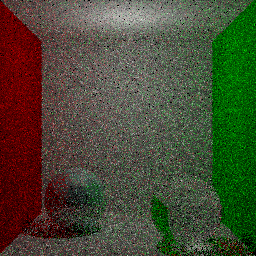
\includegraphics[width=\linewidth]{imgs/cosine_box2.png}
\caption{Uniform cosine sampling}
\end{subfigure}
\hfill
\begin{subfigure}[h]{0.4\linewidth}
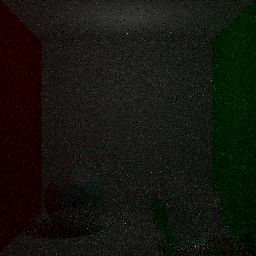
\includegraphics[width=\linewidth]{imgs/solid_angle_box2.png}
\caption{Uniform solid angle sampling}
\end{subfigure}%
\caption{Cornell Box con 2 samples per pixel}
\end{figure}

\begin{figure}
\begin{subfigure}[h]{0.4\linewidth}
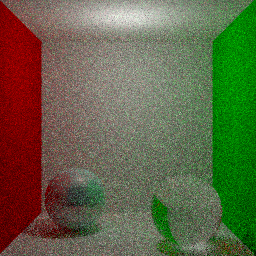
\includegraphics[width=\linewidth]{imgs/cosine_box8.png}
\caption{Uniform cosine sampling}
\end{subfigure}
\hfill
\begin{subfigure}[h]{0.4\linewidth}
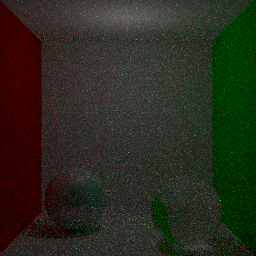
\includegraphics[width=\linewidth]{imgs/solid_angle_box8.png}
\caption{Uniform solid angle sampling}
\end{subfigure}%
\caption{Cornell Box con 8 samples per pixel}
\end{figure}

\begin{figure}
\begin{subfigure}[h]{0.4\linewidth}
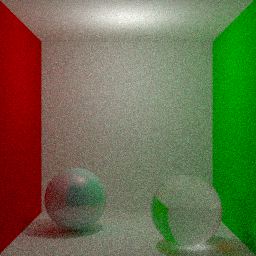
\includegraphics[width=\linewidth]{imgs/cosine_box32.png}
\caption{Uniform cosine sampling}
\end{subfigure}
\hfill
\begin{subfigure}[h]{0.4\linewidth}
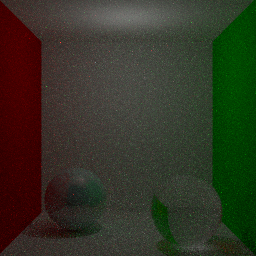
\includegraphics[width=\linewidth]{imgs/solid_angle_box32.png}
\caption{Uniform solid angle sampling}
\end{subfigure}%
\caption{Cornell Box con 32 samples per pixel}
\end{figure}

\begin{figure}
\begin{subfigure}[h]{0.4\linewidth}
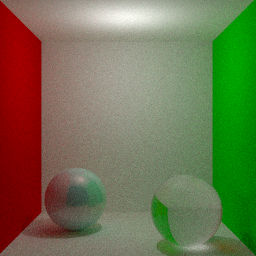
\includegraphics[width=\linewidth]{imgs/cosine_box128.png}
\caption{Uniform cosine sampling}
\end{subfigure}
\hfill
\begin{subfigure}[h]{0.4\linewidth}
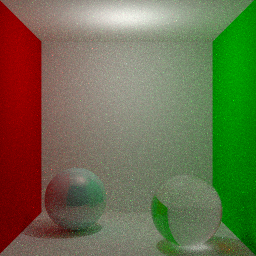
\includegraphics[width=\linewidth]{imgs/solid_angle_box128.png}
\caption{Uniform solid angle sampling}
\end{subfigure}%
\caption{Cornell Box con 128 samples per pixel}
\end{figure}

\begin{figure}
\begin{subfigure}[h]{0.4\linewidth}
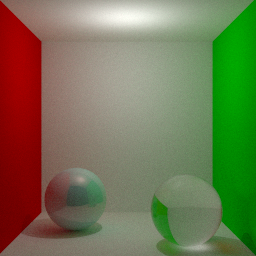
\includegraphics[width=\linewidth]{imgs/cosine_box512.png}
\caption{Uniform cosine sampling}
\end{subfigure}
\hfill
\begin{subfigure}[h]{0.4\linewidth}
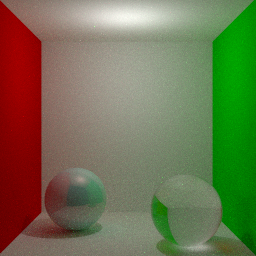
\includegraphics[width=\linewidth]{imgs/solid_angle_box512.png}
\caption{Uniform solid angle sampling}
\end{subfigure}%
\caption{Cornell Box con 512 samples per pixel}
\end{figure}

\subsection{Influencia de los materiales sobre la convergencia}

Los materiales con BRDF difusa convergen más rápido que aquellos con BRDFs
delta. En primer lugar, los materiales difusos podrán aprovechar el
\textit{next-level estimation} para calcular la contribución de las luces
puntuales en ese punto. Además el muestreo del siguiente \(\mathbf{\omega_{i}}\)
en la hemiesfera favorece la convergencia frente a un muestreo de
\(\mathbf{\omega_{i}}\) determinista.

\subsection{Fuentes de luz}
Las escenas con luces puntuales convergen significativamente más rápido que
aquellas con luces de área como se puede ver en Figuras 7-11. Este hecho se
explica dado que las luces puntuales usan \textit{next-event estimation}, que
muestrean directamente la luz de las fuentes puntuales en cada camino. En
contraste, en el caso de las luces en área, se necesitarán más caminos para que
alguno de ellos pueda explorar la dirección de la luz de área, lo que ralentiza
la convergencia.

\begin{figure}[H]
\begin{subfigure}[h]{0.4\linewidth}
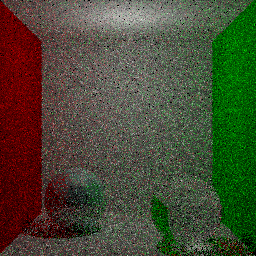
\includegraphics[width=\linewidth]{imgs/cosine_box2.png}
\caption{Luz puntual}
\end{subfigure}
\hfill
\begin{subfigure}[h]{0.4\linewidth}
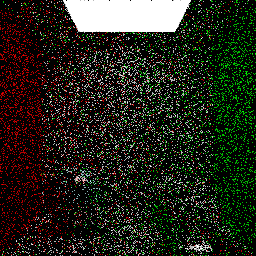
\includegraphics[width=\linewidth]{imgs/area_box2.png}
\caption{Luz de área}
\end{subfigure}%
\caption{Cornell Box con 2 samples per pixel}
\end{figure}

\begin{figure}[H]
\begin{subfigure}[h]{0.4\linewidth}
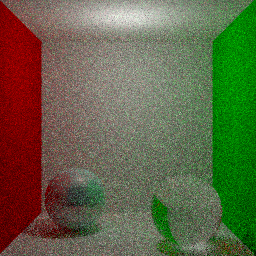
\includegraphics[width=\linewidth]{imgs/cosine_box8.png}
\caption{Luz puntual}
\end{subfigure}
\hfill
\begin{subfigure}[h]{0.4\linewidth}
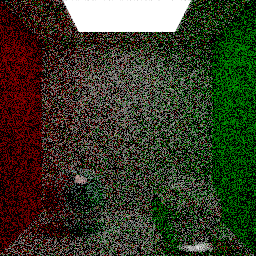
\includegraphics[width=\linewidth]{imgs/area_box8.png}
\caption{Luz de área}
\end{subfigure}%
\caption{Cornell Box con 8 samples per pixel}
\end{figure}

\begin{figure}[H]
\begin{subfigure}[h]{0.4\linewidth}
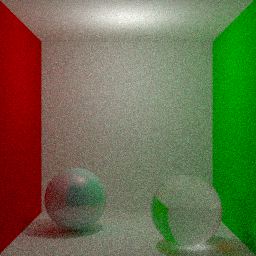
\includegraphics[width=\linewidth]{imgs/cosine_box32.png}
\caption{Luz puntual}
\end{subfigure}
\hfill
\begin{subfigure}[h]{0.4\linewidth}
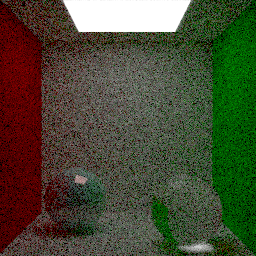
\includegraphics[width=\linewidth]{imgs/area_box32.png}
\caption{Luz de área}
\end{subfigure}%
\caption{Cornell Box con 32 samples per pixel}
\end{figure}

\begin{figure}[H]
\begin{subfigure}[h]{0.4\linewidth}
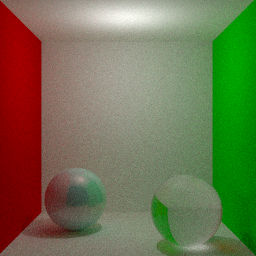
\includegraphics[width=\linewidth]{imgs/cosine_box128.png}
\caption{Luz puntual}
\end{subfigure}
\hfill
\begin{subfigure}[h]{0.4\linewidth}
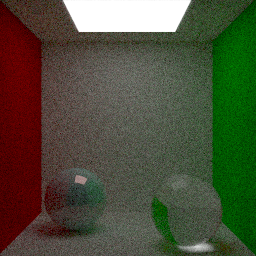
\includegraphics[width=\linewidth]{imgs/area_box128.png}
\caption{Luz de área}
\end{subfigure}%
\caption{Cornell Box con 128 samples per pixel}
\end{figure}

\begin{figure}[H]
\begin{subfigure}[h]{0.4\linewidth}
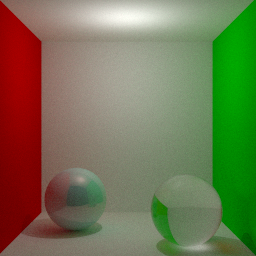
\includegraphics[width=\linewidth]{imgs/cosine_box512.png}
\caption{Luz puntual}
\end{subfigure}
\hfill
\begin{subfigure}[h]{0.4\linewidth}
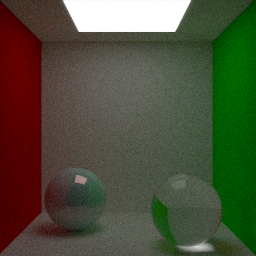
\includegraphics[width=\linewidth]{imgs/area_box512.png}
\caption{Luz de área}
\end{subfigure}%
\caption{Cornell Box con 512 samples per pixel}
\end{figure}

\newpage

\section{Iluminación global}

El algoritmo \textit{path tracer} es capaz de simular todos los cuatro effectos
de la iluminación global: \textit{hard shadows}, \textit{soft shadows},
\textit{color bleeding} y \textit{causics}. \\

Las \textbf{\textit{hard shadows}} son muy fácil de obtener con el algoritmo
\textit{path tracer}, y ya hemos visto como lucen en las Figuras 2-6, basta con
añadir a la escena luces puntuales. \\

Las \textbf{\textit{soft shadows}} son muy fácil de obtener también. Figuras
7-11, y basta con añadir a la escena alguna luz de area. \\

\begin{figure}[H]
\begin{subfigure}[h]{0.4\linewidth}
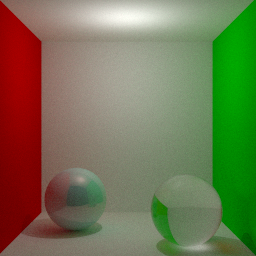
\includegraphics[width=\linewidth]{imgs/hard.png}
\caption{Hard shadow}
\end{subfigure}
\hfill
\begin{subfigure}[h]{0.4\linewidth}
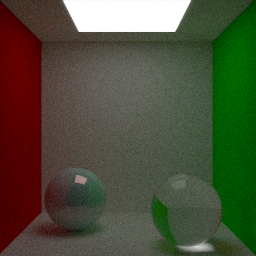
\includegraphics[width=\linewidth]{imgs/soft.png}
\caption{Soft shadow}
\end{subfigure}
\caption{Comparativa de sombras}
\end{figure}

\textbf{\textit{Color bleeding}} es el fenómeno por el cual una superficie es
coloreada por el color reflejado de otra superficie cercana. También es muy
fácil de conseguir, basta con colocar dos objectos cerca uno del otro. Se puede
ver en las paredes de la caja de las Figuras 2-11 o con más claridad en la
Figura 13 tanto en la pared de atrás, en el suelo, en la cara o en la espalda
del conejo de plástico. \\

\begin{figure}[H]
\centering
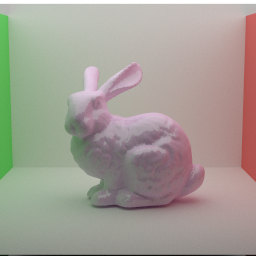
\includegraphics[width=0.6\linewidth]{imgs/plastic_bunny.png}
\caption{Conejo de plástico}
\end{figure}

Finalmente las \textbf{\textit{cáusticas}} son algo más difícil de conseguir ya
que al tratarse de rayos de luz muy concentrados en un punto, es poco probable
que el algoritmo genere estos caminos eficientemente. Sin embargo con un gran
numero de \textit{samples per pixel}, la geometría y la iluminación correcta se
puede conseguir: TODO CAMBIAR imagen
\begin{figure}[H]
\centering
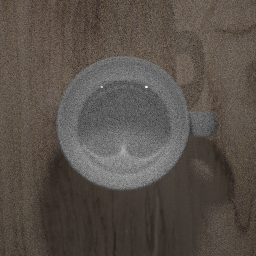
\includegraphics[width=0.6\linewidth]{imgs/nephroid.png}
\caption{Taza de cerámica (difusa + especular) (medio metida en una mesa) en la
  que se puede ver una cáustica nefroide}
\end{figure}

\section{Extensiones}
TODO

\end{document}
